\documentclass[UTF8,a4paper,12pt]{article}

\usepackage[version=3]{mhchem} % Package for chemical equation typesetting
\usepackage{ctex}
\usepackage{siunitx} % Provides the \SI{}{} and \si{} command for typesetting SI units
\usepackage{graphicx} % Required for the inclusion of images
\usepackage{natbib} % Required to change bibliography style to APA
\usepackage{amsmath} % Required for some math elements
\usepackage{enumitem}
\usepackage{indentfirst}

\usepackage[top=2cm, bottom=2cm, left=2cm, right=2cm]{geometry}
\usepackage{algorithm}
\usepackage{algorithmicx}
\usepackage{algpseudocode}

\renewcommand{\labelenumi}{\alph{enumi}.} % Make numbering in the enumerate environment by letter rather than number (e.g. section 6)
\floatname{algorithm}{算法}
\renewcommand{\algorithmicrequire}{\textbf{输入:}}
\renewcommand{\algorithmicensure}{\textbf{输出:}}

\usepackage{listings}

\usepackage{tikz}
\usetikzlibrary{shapes.geometric, arrows}

\usepackage{listings}
\usepackage{subfigure}
% \usepackage{times} % Uncomment to use the Times New Roman font
%----------------------------------------------------------------------------------------
%	DOCUMENT INFORMATION
%----------------------------------------------------------------------------------------

\begin{document}

\begin{titlepage}
    \begin{center}
        \phantom{Start!}
    	  \vspace{2cm}
        \center{\zihao{1} 中山大学数据科学与计算机学院}
        \center{\zihao{1} 计算机科学与技术专业-人工智能}
        \center{\zihao{1} 本科生实验报告}
        \center{(2018-2019学年秋季学期)}
        {
            \setlength{\baselineskip}{40pt}
            \vspace{1cm}
            \zihao{-2}
            \center{
                \begin{tabular}{cc}
              	学\qquad 号:& \underline{~~~~~~16337113~~~~~~}  \\
              	姓\qquad 名:& \underline{~~~~~~~劳马东~~~~~~~}  \\
                教学班级:   & \underline{~~~~~教务2班~~~~~}  \\
              	专\qquad 业:& \underline{~~~~~~~~~超算~~~~~~~~}  \\
              	\end{tabular}
            }
        }
    \end{center}
\end{titlepage}

\section{实验内容}
\subsection{算法原理}
\subsubsection{GBDT回归树}
\begin{enumerate}[itemindent=0.5em,label=\arabic*、]
  \item 概述
  \par \qquad GBDT(Gradient Boosting Decision Tree)是一种迭代的决策树算法,该算法由多棵决策树组成,所有树的结论累加起来做最终答案。
  其核心就在于,每一棵树学的是之前所有树结论累加和的残差,即与真实结论的差,形式化的定义为:
  \begin{equation}
    \begin{aligned}
      Y^{i} &= Y_{true} - \sum_{k=0}^{i-1}Y^k_{predict}\ ,\ i \ge 0
    \end{aligned}
  \end{equation}
  \par \qquad 比如A的真实年龄是18岁,但第一棵树的预测年龄是12岁,差了6岁,即残差为6岁。那么在第二棵树里我们把A的年龄设为6岁去学习,
  如果第二棵树真的能把A分到6岁的叶子节点,那累加两棵树的结论就是A的真实年龄;如果第二棵树的结论是5岁,则A仍然存在1岁的残差,
  第三棵树里A的年龄就变成1岁,继续学,以此类推,直到残差小到一定程度。

  \item 训练过程
    \begin{enumerate}[itemindent=0.5em,label=(\arabic*)]
      \item 初始化残差$E_0$为$Y$, $i$为0;
      \item 增加一棵决策树$T_i$在数据集$(X, E_i)$上训练;
      \item $T_i$预测$X$得到预测值$Y^i_{predict}$;
      \item 计算新的残差$E_{i+1}=E_i - Y^i_{predict}$;
      \item 如果残差收敛,迭代结束,否则$i$增加1,回到第2步。
    \end{enumerate}

  \item Shrinkage
  \par \qquad Shrinkage(缩减)的思想认为,每次走一小步逐渐逼近结果的效果,要比每次迈一大步很快逼近结果的方式更容易避免过拟合。
即它不完全信任每一个棵残差树,它认为每棵树只学到了真理的一小部分,累加的时候只累加一小部分,通过多学几棵树弥补不足,
具体到公式,就是:
  \begin{equation}
    E_{i+1}=E_i - \theta \times Y^i_{predict}
  \end{equation}
  其中$\theta$是缩减率,也叫学习率、可信度。
\item 预测过程
\par \qquad 预测的过程就是把所有决策树的结果累加的过程,即:
\begin{equation}
  Y_{predict} = \sum_{i=0}^{n}(\theta \times Y^i_{predict})
\end{equation}
\end{enumerate}
\subsubsection{逻辑回归}
\begin{enumerate}[itemindent=0.5em,label=\arabic*、]
  \item 概述
  \par \qquad 二元逻辑回归是计算在给定$x$的情况下,属于某类的概率,即:
  \begin{equation}
    f(x) = P(label|x) \in [0, 1]
  \end{equation}
  \par \qquad 它属于一种线性算法,即$x$的每个维度的最高次幂都是1。特征向量$x$的每一个维度,都会对结果产生影响,
  所以我们希望可以给每一个特征赋予一个权重来计算结果:
  \begin{equation}
    s = w_0 + \sum_{i=1}^d (w_i \times x_i)
  \end{equation}
  表达式中的$w_i$表示第$i$维特征的权重,$w_i>0$表示该特征对正类别有正面影响,且值越大,正面影响越大,反之亦然。
  \par \qquad 问题是这样计算出来的$s$取值是$(-\infty, +\infty)$而不是一个概率值,因此需要一种转换——$sigmoid$函数。
  \begin{equation}
    g(z) = \frac{1}{1 + e^{-z}}
  \end{equation}
  其函数曲线如图1,在$z \rightarrow -\infty$时,其取值为0,$z \rightarrow +\infty$时取值为1,在远离0的地方函数值
  越接近0或1,函数值为0.5是一种不可区分的状态。
  \begin{figure}[h]
  \begin{center}
  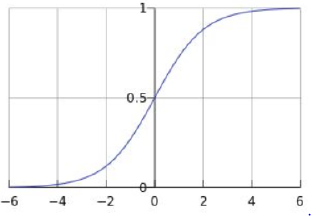
\includegraphics[width=0.4\textwidth]{sigmoid.png} % Include the image placeholder.png
  \caption{sigmoid函数图像}
  \end{center}
  \end{figure}
  \par \qquad 因此,$f(x)$实际上是一个复合函数,为:
  \begin{equation}
    f(x) = g(s) = g(w\widetilde{x}) = \frac{1}{1 + e^{-w\widetilde{x}}} \in (0, 1)
  \end{equation}
  其中$\widetilde{x}$表示特征向量$x$加上第0维的1后的增广向量,即$\widetilde{x} = (1, x_1, x_2, ..., x_d)$。
  \item 训练过程
  \par \qquad 训练过程就是计算得到$w$的过程。假设有一个基于sigmoid函数的损失函数$e(w)$是关于$w$的函数,
  我们的目标是使预测值与真实值的误差最小,即$e(w)$取最小值,对应的$w$即为所求。在数学上,可以通过求导的方法计算极小值点,
  进而得到最小值点,但问题是很多损失函数难以求导,因此需要用到梯度下降法。
  \par \qquad 梯度下降法最终的目标是让$w$走到$e(w)$导数为0的地方。假设$e(w)$是一个开口向上的函数,
  如果当前$w$处在右半边,即$e^{'}(w)>0$,那么$w$就应该往左走;如果$w$在左半边,即$e^{'}(w)<0$,那么$w$就应该往右走,
  不断重复直到$e^{'}(w)=0$。
  \item 预测过程
  \par \qquad 预测过程很简单,得到$w$之后,计算$f(x)$,如果概率大于0.5,认为属于正类别,小于0.5属于负类别,等于0.5不可区分或者归到某一类别中。
  \item 从二元到多元——oneVSall
  \par \qquad 假设数据集一共有n类,分别记为$L1, L2, ..., L_n$,oneVSall的做法是每次取一个类别$L_i$作为正类别,其余类别全部
  作为负类别,将其输入到逻辑回归模型中训练,这样得到一组权重$W_i$。重复这个过程n次,就能得到n组权重,记为
  $W_1, W_2, ..., W_n$,这就是整个训练过程。
  \par \qquad 在预测时,同样是每次选择一个类别作为正类别,用逻辑回归的方法
  得到一个预测概率$p_i$,特征向量$x$的类别是这些概率的最大值对应的类别,即:
  \begin{equation}
    f(x) = \arg\max_{i}\frac{1}{1+e^{-W_i\widetilde{x}}}
  \end{equation}
\end{enumerate}

\subsection{伪代码}
\begin{enumerate}[itemindent=0.5em,label=\arabic*、]
  \item GDBT训练过程
  \begin{algorithm}
        \begin{algorithmic}[1] %每行显示行号
            \Require 训练集$X$,训练集$y$, 学习率$\theta$
            \Ensure 训练好的多棵决策树
            \Function {$fit$}{$X, y, \theta$}
                \State $T \gets\ collection\ of\ dicision\ trees$
                \State $E_{new} \gets y$
                \State $i \gets 0$
                \Repeat
                  \State $E \gets E_{new}$
                  \State $T_i \gets\ new\ dicision\ tree$
                  \State $T_i.fit(X, E)$
                  \State $Y^i_p \gets T_i.predict(X)$
                  \State $E_{new} \gets E - \theta \times Y^i_p$
                  \State $i \gets i + 1$
                \Until {$E_{new}\ is\ not\ convergent$}
                \State\Return {$T$}
            \EndFunction
        \end{algorithmic}
    \end{algorithm}

    \newpage
    \item logistic回归训练过程
    \begin{algorithm}
          \begin{algorithmic}[1] %每行显示行号
              \Require 训练集$X(m \times n)$,训练集$y$, 学习率$\theta$, 损失函数$E$
              \Ensure 收敛的权重
              \Function {$fit$}{$X, y, \theta$}
                  \State $a\_X \gets argmented(X)$
                  \State $W_{new} \gets array\ of\ n+1\ random\ value$
                  \Repeat
                    \State $W \gets W_{new}$
                    \State $W_{new} = W - \theta \times \frac{\partial{E(W)}}{\partial{W}}$
                  \Until{$W_{new}\ is\ convergent$}
                  \State\Return {$W_{new}$}
              \EndFunction
          \end{algorithmic}
      \end{algorithm}

      \item oneVSall训练过程
      \begin{algorithm}
            \begin{algorithmic}[1] %每行显示行号
                \Require 训练集$X(m \times n)$,训练集$y$
                \Ensure 对应每个类别训练好的二元分类模型
                \Function {$fit$}{$X, y$}
                    \State $clfs \gets\ collection\ of\ binary\ classifiers$
                    \For{$label \in unique(y)$}
                        \State $y\_new \gets to\_binary(y, label)$
                        \State $clfs_i \gets\ new\ binary\ classifier$
                        \State $clfs_i.fit(X, y\_new)$
                    \EndFor
                    \State\Return {$clfs$}
                \EndFunction
            \end{algorithmic}
        \end{algorithm}
\end{enumerate}

\subsection{关键代码}
\begin{enumerate}[itemindent=0.5em,label=\arabic*、]
  \item GBDT训练
  \par \qquad 在实际情况下,残差是很难收敛的,因此为了避免无限迭代,需要设置残差的阈值或决策树的数量,二者的
  效果是等价的。
  \par \qquad 图2的代码中$n\_estimators$是决策树的数量,$RegressionTree$是$CART$树,其三个参数用于
  剪枝。
  \begin{figure}[h]
  \begin{center}
  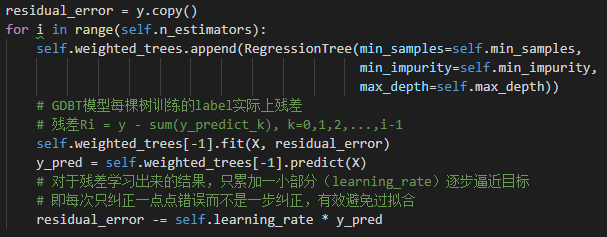
\includegraphics[width=0.8\textwidth]{train.png} % Include the image placeholder.png
  \caption{GBDT训练}
  \end{center}
  \end{figure}
  \item GBDT预测
  \par \qquad 预测是训练的逆过程,训练时每棵树的预测结果只才用了一小部分,因此预测时也应该如此。
  \par \qquad 图3代码中,$map$函数将每棵树映射为其预测结果乘上学习率,这可以提高并行度,减少预测时间。
  每棵树的预测结果的累加和组成了最终的预测结果。
  \begin{figure}[h]
  \begin{center}
  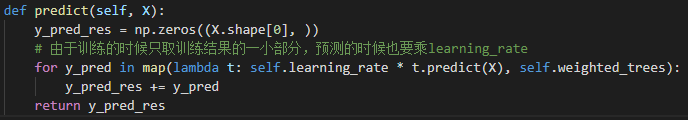
\includegraphics[width=0.8\textwidth]{predict.png} % Include the image placeholder.png
  \caption{GBDT预测}
  \end{center}
  \end{figure}

  \item 逻辑回归训练
  \par \qquad 判断是否收敛的方法有两种,一种是判断权重向量本身,另一种是判断损失函数值是否达到一定阈值。项目中使用了后者。
  \par \qquad 代码如图4。$argmented$函数在$X$每一行的第一个位置插入一个1,返回增广的$X$,简单起见权重向量
  $W$被初始化为全0;以交叉熵$cross\_entropy$作为损失函数,其导数$gradient\_ce$
  作为梯度函数;函数$fmin\_tnc$使用梯度下降法优化$W$直到收敛。
  \begin{figure}[h]
  \begin{center}
  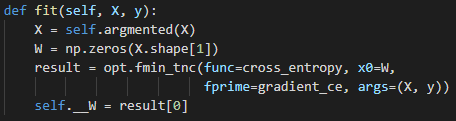
\includegraphics[width=0.6\textwidth]{log_fit.png} % Include the image placeholder.png
  \caption{逻辑回归训练}
  \end{center}
  \end{figure}

  \item oneVSall预测
  \par \qquad 如图5,在预测过程中需要记录两个量:当前的预测结果$y\_pred$及其对应的概率$y\_prob$,
  预测时遍历每个类别$c$,用这个类别对应的分类器来预测$X$得到一个结果$y\_p$,这个结果是概率数组而不是
  类别数组。有了$y\_p$和$y\_prob$,就能比较他们对应位置的元素,如果$y\_p$的概率比$y\_prob$大,就应该
  更新$y\_prob$和$y\_pred$。
  \begin{figure}[h]
  \begin{center}
  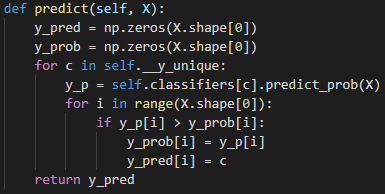
\includegraphics[width=0.55\textwidth]{onevsall-predict.png} % Include the image placeholder.png
  \caption{oneVSall预测}
  \end{center}
  \end{figure}
\end{enumerate}

\section{创新点$\&$优化}
\subsection{GBDT回归树}
\begin{enumerate}[itemindent=0.5em,label=\arabic*、]
  \item $tag$处理
  \begin{enumerate}[itemindent=0.5em,label=(\arabic*)]
    \item 基于频数
    \par 不同的tag有1996个,数据集总共80000行,挑选出其中出现次数超过一定阈值的tag作为特征。
    实验中发现阈值为5000时最佳,最终挑选出的tag如图(a)。
    \begin{figure}[H]
    \centering
    \subfigure[频数超过5000的tag]{
    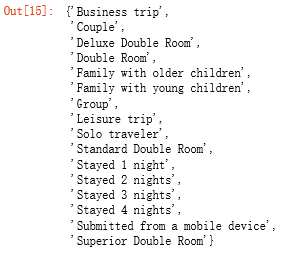
\includegraphics[width=0.4\textwidth]{tag-5000.png}}
    \subfigure[效果最好的22个tag]{
    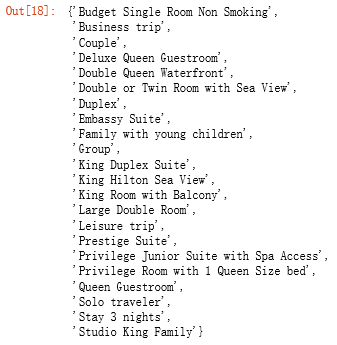
\includegraphics[width=0.4\textwidth]{tag-best.png}}
    \end{figure}
    \item 基于效果
    \par 最直接的方法就是将tag逐个有放回地加入到属性中,观察其对最终验证集相关系数的影响,
    选出最优的一些。实验中有选择地对一些tag做了测试,最终挑选的22个最好的tag如图(b)。
    \item 基于类别
    \par 仔细分析tag可以发现可以大致分为以下几类:
    \begin{enumerate}
      \item Leisure or Business Trip
      \item number of people
      \item room
      \item stay n nights
      \item submitted from a mobile device or not
    \end{enumerate}
    这五类tag可以作为五个特征,给每一行数据在该特征上赋予特定的值(如Leisure Trip为0、
    Business Trip为1,solo为1、couple为2、family with young children为3等)。
  \end{enumerate}
  \item 优化数据分布不均的问题
  \par \qquad 查看y的分布,会发现数据是极度右偏的,如下图(c)。而许多回归模型都假设数据是
  正态分布的,因此需要将偏态分布转化为正态分布,常用的方法是box-cox变换。
    \begin{equation}
      y(\lambda)=
      \begin{cases}
       \ln(y)& \lambda =0\\
       \frac{y^{\lambda} - 1}{\lambda}& \lambda \neq 0
      \end{cases}
    \end{equation}
    式中$y(\lambda)$为经Box-Cox变换后得到的新变量,$y$为原始连续因变量,要求取值为正,$\lambda$为变换参数。
    项目中使用了scipy库的box-cox函数,其返回$\lambda$的值和变换后的$y$。利用该$\lambda$值能得到逆变换后的$y$,即:
    \begin{equation}
      y=
      \begin{cases}
       e^{y(\lambda)}& \lambda =0\\
       (y(\lambda) \times \lambda + 1)^{\frac{1}{\lambda}}& \lambda \neq 0
      \end{cases}
    \end{equation}

  \begin{figure}[H]
  \centering
  \subfigure[y的分布]{
  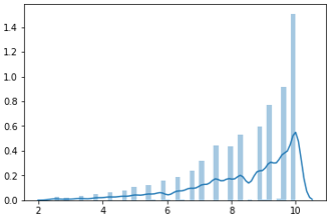
\includegraphics[width=0.4\textwidth]{y.png}}
  \subfigure[box-cox+标准正态转化-y的分布]{
  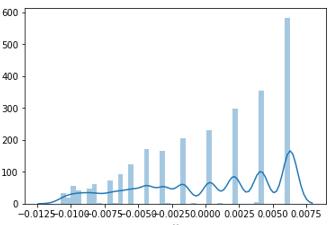
\includegraphics[width=0.4\textwidth]{y-dc.png}}
  \end{figure}

  \item 特征筛选
  \par 计算各个特征与y的pearson相关系数(如图3,已取绝对值),从中删除一些相关性较低的tag类别。
  可以看到Total\_Number\_of\_Reviews\_Reviewer\_Has\_Given和mobile\_device两个特征
  相关性极低,可以删除。
  \begin{figure}[h]
  \begin{center}
  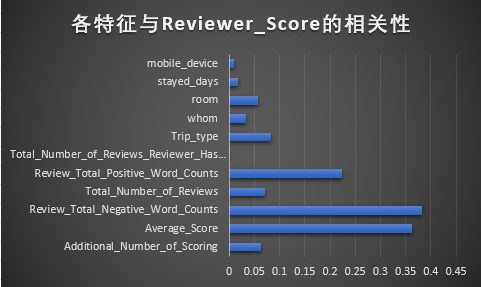
\includegraphics[width=0.5\textwidth]{feature-pear.png}
  \caption{各特征与y的相关系数}
  \end{center}
  \end{figure}
\end{enumerate}
\subsection{doc2vec而不是word2vec}
\par word2vec可以将词转化为一个K维的向量,而段落/文本的向量就是其含有的词对应的向量的均值,
因此段落/文本之间的相似性也就转化为向量之间的距离(如余弦距离、欧氏距离)。
\par 然而,即使上述模型对词向量进行平均处理,我们仍然忽略了单词之间的排列顺序对情感分析的影响。
因为word2vec只是基于“词”的维度进行语义分析,而并不具有“上下文”的语义分析能力。
Quoc Le和Tomas Mikolov提出了Doc2Vec方法,该方法在word2vec的基础上增加一个段落向量,
使用一个paragraph\ id增强了同一段落之间不同句子之间的联系,从而具有“上下文”语义分析的能力。

\section{实验结果及分析}
\subsection{实验结果展示}
\begin{enumerate}[itemindent=0.5em,label=\arabic*、]
  \item GBDT回归树
  取实验数据训练集的前16行作为训练集,16-21行作为测试集,如下图(a)、(b)、(d):
  \begin{figure}[H]
  \centering
  \subfigure[训练集]{
  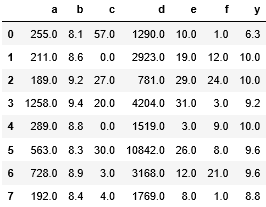
\includegraphics[width=0.4\textwidth]{result-train.png}}
  \subfigure[训练集]{
  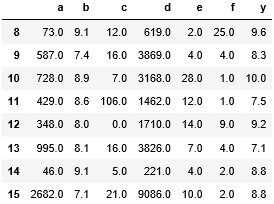
\includegraphics[width=0.4\textwidth]{result-train2.png}}
  \end{figure}
  使用300棵CART树,学习率为0.065,CART树的最大深度为3。训练过程中残差均值的变化趋势如下图
  (c),一开始时残差减小较快,在迭代100次之后基本趋于0。用训练好的模型预测测试集,结果如图(d)
  $y\_pred$,计算得相关系数为0.96:
  \begin{figure}[H]
  \centering
  \subfigure[训练过程残差均值变化]{
  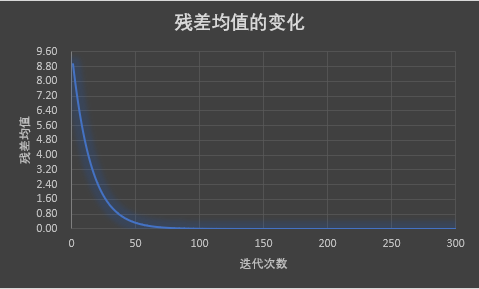
\includegraphics[width=0.3\textwidth]{gbdt-errors.png}}
  \subfigure[测试集与预测结果]{
  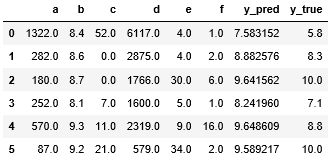
\includegraphics[width=0.4\textwidth]{result-test.png}}
  \end{figure}
  \item 逻辑回归
  \par 训练集如下,含有两个特征,分别是两门考试的成绩,$y$为是否通过。
  \begin{figure}[H]
  \centering
  \subfigure[训练集]{
  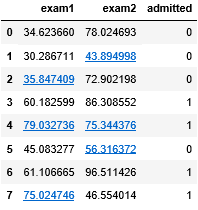
\includegraphics[width=0.25\textwidth]{result-log-train.png}}
  \subfigure[训练集]{
  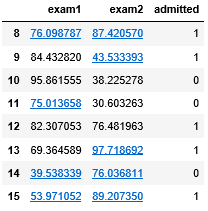
\includegraphics[width=0.25\textwidth]{result-log-train2.png}}
  \end{figure}
  使用交叉熵作为损失函数,其导数作为梯度函数,调用scipy.optimize模块的fmin\_tnc函数训练,
  期间交叉熵的变化情况如下图(g),一开始时错误减小较快,在第9次迭代之后基本稳定在0.2327左右。
  得到的权重向量$W$为:$(-18.66001375,0.14838242,0.14839205)$,预测结果如下图(h):
  \begin{figure}[H]
  \centering
  \subfigure[训练过程交叉熵变化]{
  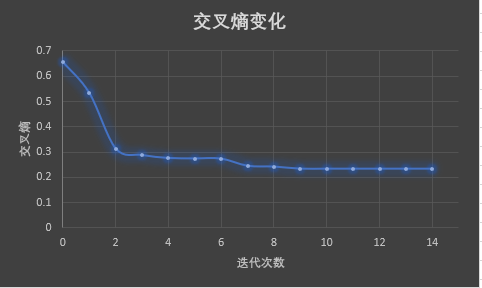
\includegraphics[width=0.35\textwidth]{log-errors.png}}
  \subfigure[测试集与预测结果]{
  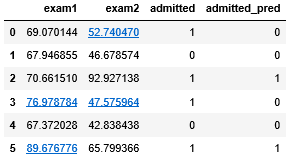
\includegraphics[width=0.4\textwidth]{result-log-test.png}}
  \end{figure}
\end{enumerate}

\newpage
\subsection{评测指标展示及分析}
\subsubsection{GBDT回归树}
\begin{enumerate}[itemindent=0.5em,label=\arabic*、]
  \item 相关系数
  \par \qquad 使用300棵CART树,学习率为0.065,CART树的最大深度为3。采用5折交叉验证,
  分别评测基本数据集和各种数据集处理方法在验证集上的相关系数以及上交后在测试集上的相关系数,
  结果如下表。
  \par \qquad 不同的优化方法在验证集和测试集上都得到了不同程度的提升。
  基于频数的处理方法提升最小,这是因为出现次数多的tag区分能力不强;
  基于类别的方法在测试集上达到了一个新的数量级——0.66,因为这种方法给每行数据的赋值是有意义的,
  值的大小能体现tag在某一类tag中的重要程度;基于效果的处理方法在测试集上效果最好,这毋庸置疑,
  它本身就是从模型出发,挑选出对模型提升最有利的tag;box-cox变换无论在验证集和测试集没有达到预期的效果,
  初步认为是测试集上y的分布和训练集不一致导致的。
  \begin{center}
    \begin{tabular}{ccc}
    \hline
    优化方法 & 验证集相关系数 & 测试集相关系数\\
    - & 0.6538 & 0.6540\\
    tag处理-基于频数 & 0.6575 & 0.6575\\
    tag处理-基于类别 & 0.6574 & 0.6614\\
    tag处理-基于效果 & 0.6572 & 0.6616\\
    基于效果+box-cox变换 & 0.6575 & 0.6598\\
    \hline
    \end{tabular}
  \end{center}
  \item 预测y与原始y的分布
  \par \qquad 我们的目标是使预测出来的y(记为$y_p$)与训练集上y(记为$y_t$)分布尽可能一致。
  \par \qquad 在不做任何变换之前,预测的y(记为$y^0_p$)与$y_t$分布差别较大——$y_t$是极度右偏的,
  左边几乎没有分布,而$y^0_p$在左边部分明显过多;
  \par \qquad 经过box-cox变换后,预测的y(记为$y^{bc}_p$)依然极度右偏,但是左边的分布明显减少,与$y_t$基本一致。
  \begin{figure}[H]
  \centering
  \subfigure[$y_t$的分布]{
  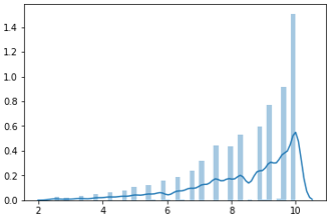
\includegraphics[width=0.3\textwidth]{y.png}}
  \subfigure[无变换-$y^0_p$的分布]{
  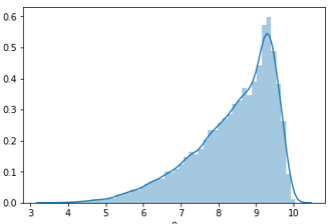
\includegraphics[width=0.3\textwidth]{y-pred.png}}
  \subfigure[box-cox变换-$y^{bc}_p$的分布]{
  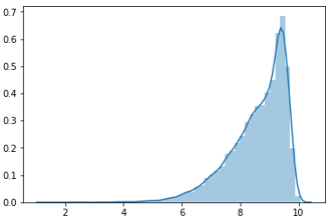
\includegraphics[width=0.3\textwidth]{y-pred-bc.png}}
  \end{figure}
\end{enumerate}
\subsubsection{分类问题——逻辑回归}
\begin{enumerate}[itemindent=0.5em,label=\arabic*、]
  \item 准确率
  \par \qquad 实验中对比了两种文本转向量方法——word2vec和doc2vec。word2vec使用的模型是glove官网提供的glove.840B.300d.txt;
  doc2vec使用的是自己训练的模型,参数window=5, vector\_size=150, negative=25, epochs=25, alpha=0.05。
  \par \qquad 最终两者5折交叉验证的准确率如下表。在二分类问题中,doc2vec相对于word2vec提高了将近2\%,效果明显;而在五分类问题中,
  doc2vec准确率低于word2vec,猜测原因是类别多了之后段与段之间的联系不再那么紧密,doc2vec模型转换得到的文本向量与原文本的意思有较大出入。
  \begin{center}
    \begin{tabular}{ccc}
    \hline
    方法 & 二分类验证集准确率 & 五分类验证集准确率\\
    word2vec & 0.8714 & 43.3266\\
    doc2vec & 0.8901 & 43.3101\\
    \hline
    \end{tabular}
  \end{center}
\end{enumerate}
\end{document}
